\documentclass[12pt,a4paper,oneside]{article}
\usepackage[colorlinks=true,unicode]{hyperref}
\usepackage[utf8]{inputenc}
\usepackage[czech]{babel}
\usepackage{graphicx}
\usepackage{pdfpages}
\textwidth 16cm \textheight 25cm
\topmargin -1.3cm 
\oddsidemargin 0cm
\usepackage{footnote}
\pagestyle{empty}
\begin{document}
\title{Šablona MLAB}
\author{Jakub Kákona, kaklik@mlab.cz}
\maketitle

\thispagestyle{empty}
\begin{abstract}
Modul řeší problém připojení dlouhých vedení k citlivým modulům stavebnice. Obsahuje přepěťovou ochranu a možnost svodu napětí ze stínění kabelu. 
\end{abstract}

\begin{figure} [htbp]
\begin{center}
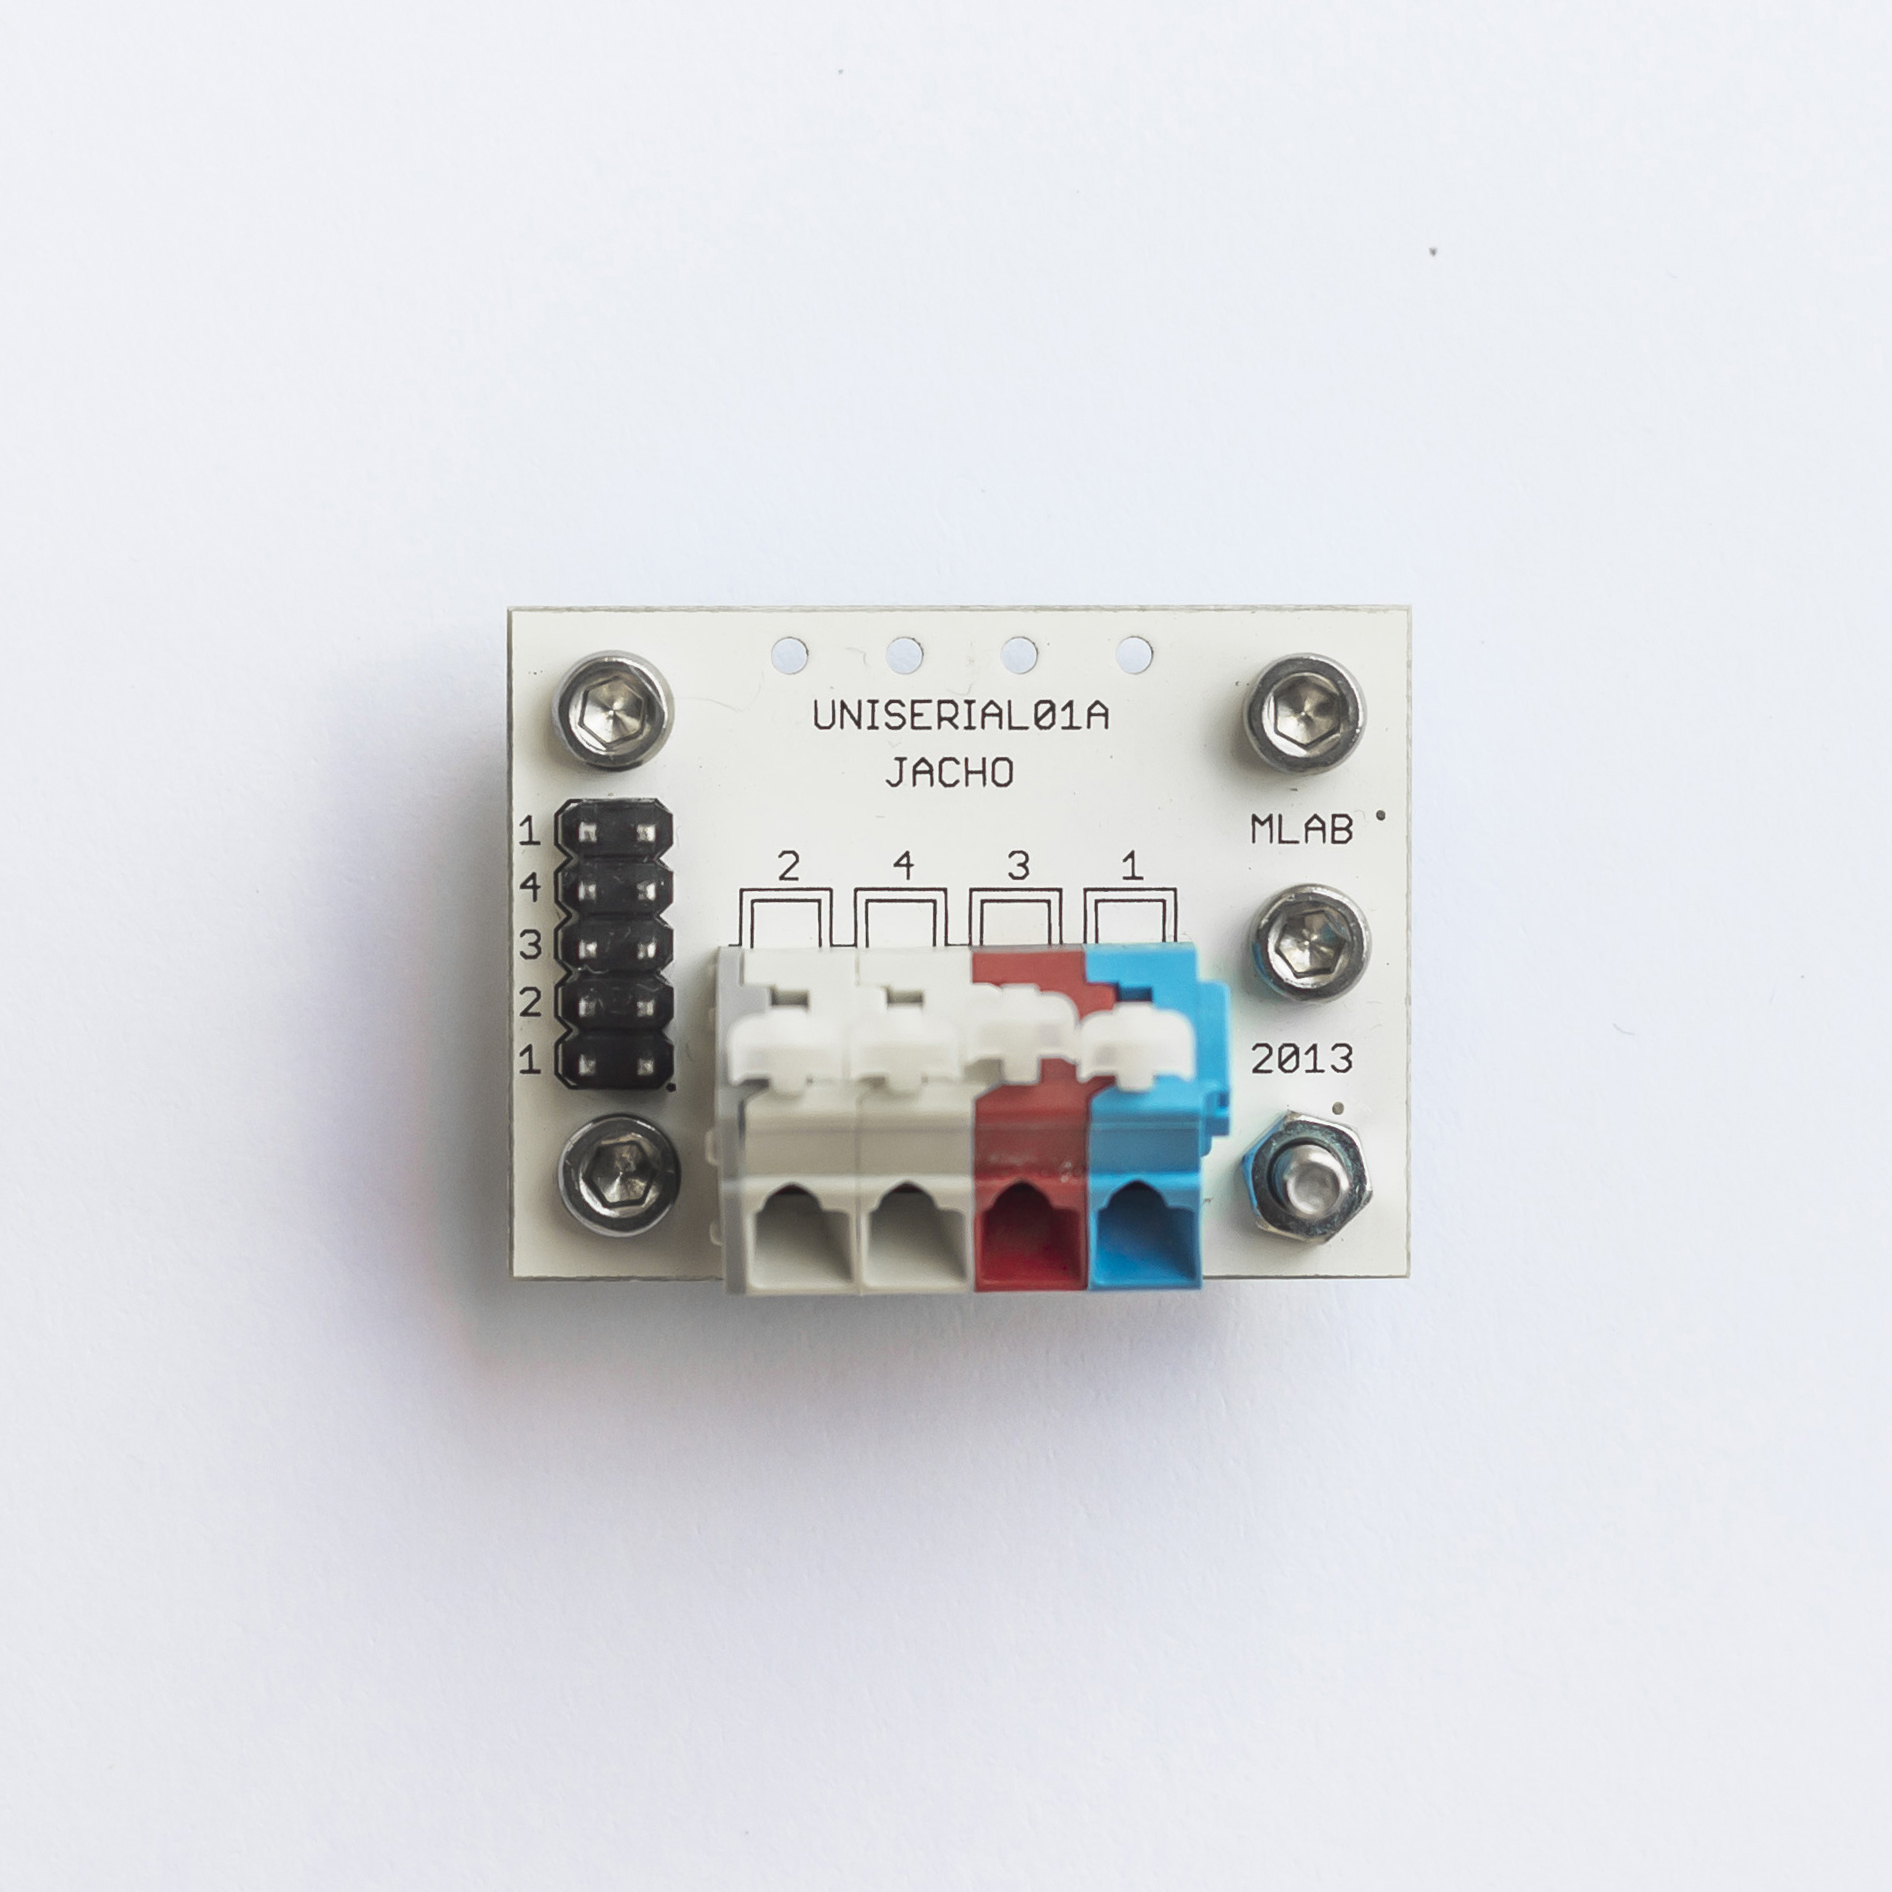
\includegraphics [width=80mm] {./img/UNISERIAL01A_Top_Big.JPG} 
\end{center}
\end{figure}

\begin{figure} [b]

\includegraphics [width=25mm] {./img/UNISERIAL01A_QRcode.png} 
\end{figure}

\newpage
\tableofcontents


\section{Technické parametry}
\begin{table}[htbp]
\begin{center}
\begin{tabular}{|c|c|c|}
\hline
\multicolumn{1}{|c|}{Parametr} & \multicolumn{1}{|c|}{Hodnota} & \multicolumn{1}{|c|}{Poznámka} \\ \hline
Napájecí napětí & max +5V &  500mA \\ \hline
Digitální signály &  3,3 V nebo 5 V &  Podle typu osazených diod \\ \hline\end{tabular}
\end{center}
\end{table}

\newpage

\section{Popis konstrukce}

\subsection{Zapojení}

\begin{figure} [h!tbp]
  \centering
  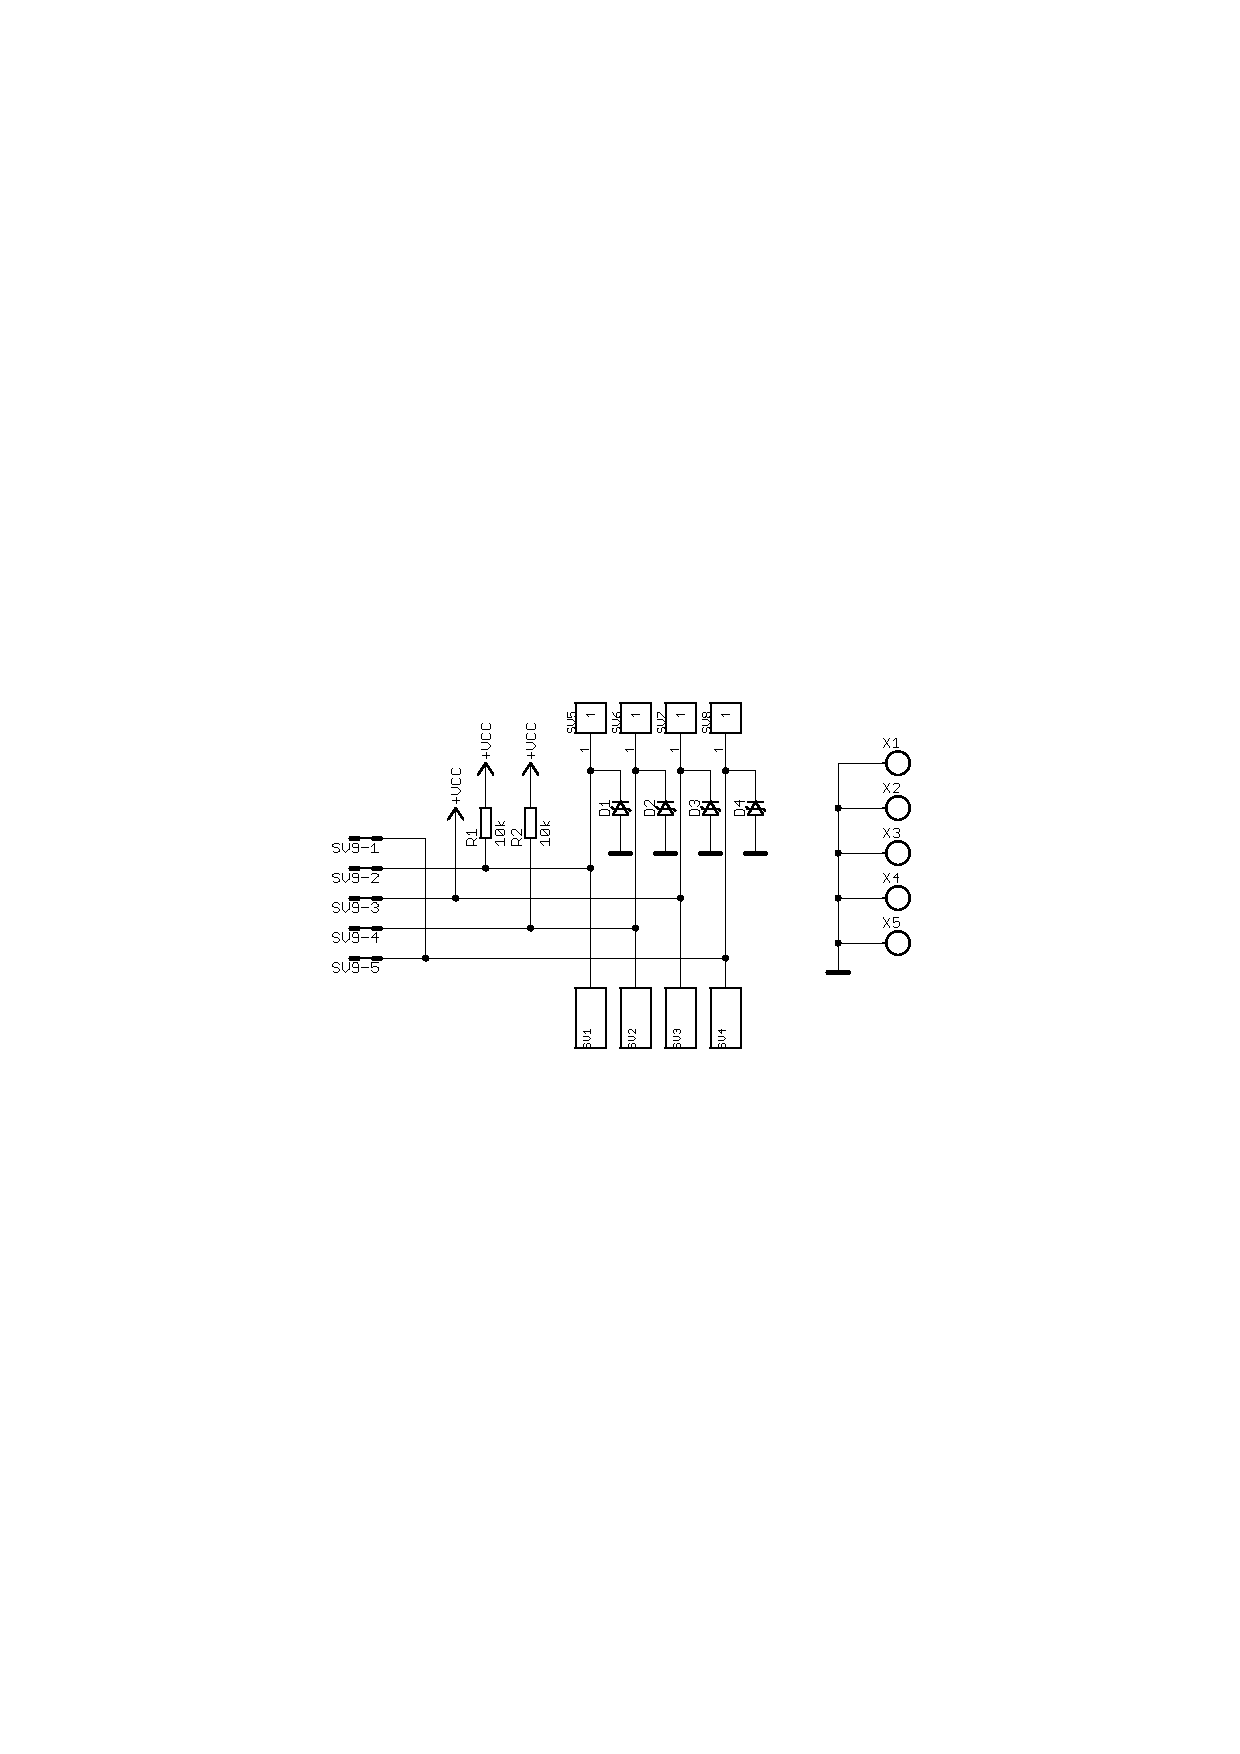
\includegraphics[trim = 5.0cm 11.5cm 5.0cm 11.5cm, clip, width=10cm]{../../CAM_DOC/SCH.pdf}
  \caption{Osazovací plán horní a spodní strany plošného spoje}
  \label{fig:osazovaci_plan}
\end{figure}

\subsection{Odrušení}

\subsection{Mechanická konstrukce}

\section{Výroba a testování}

\subsubsection{Osazení}

\begin{figure} [h!tbp]
  \centering
  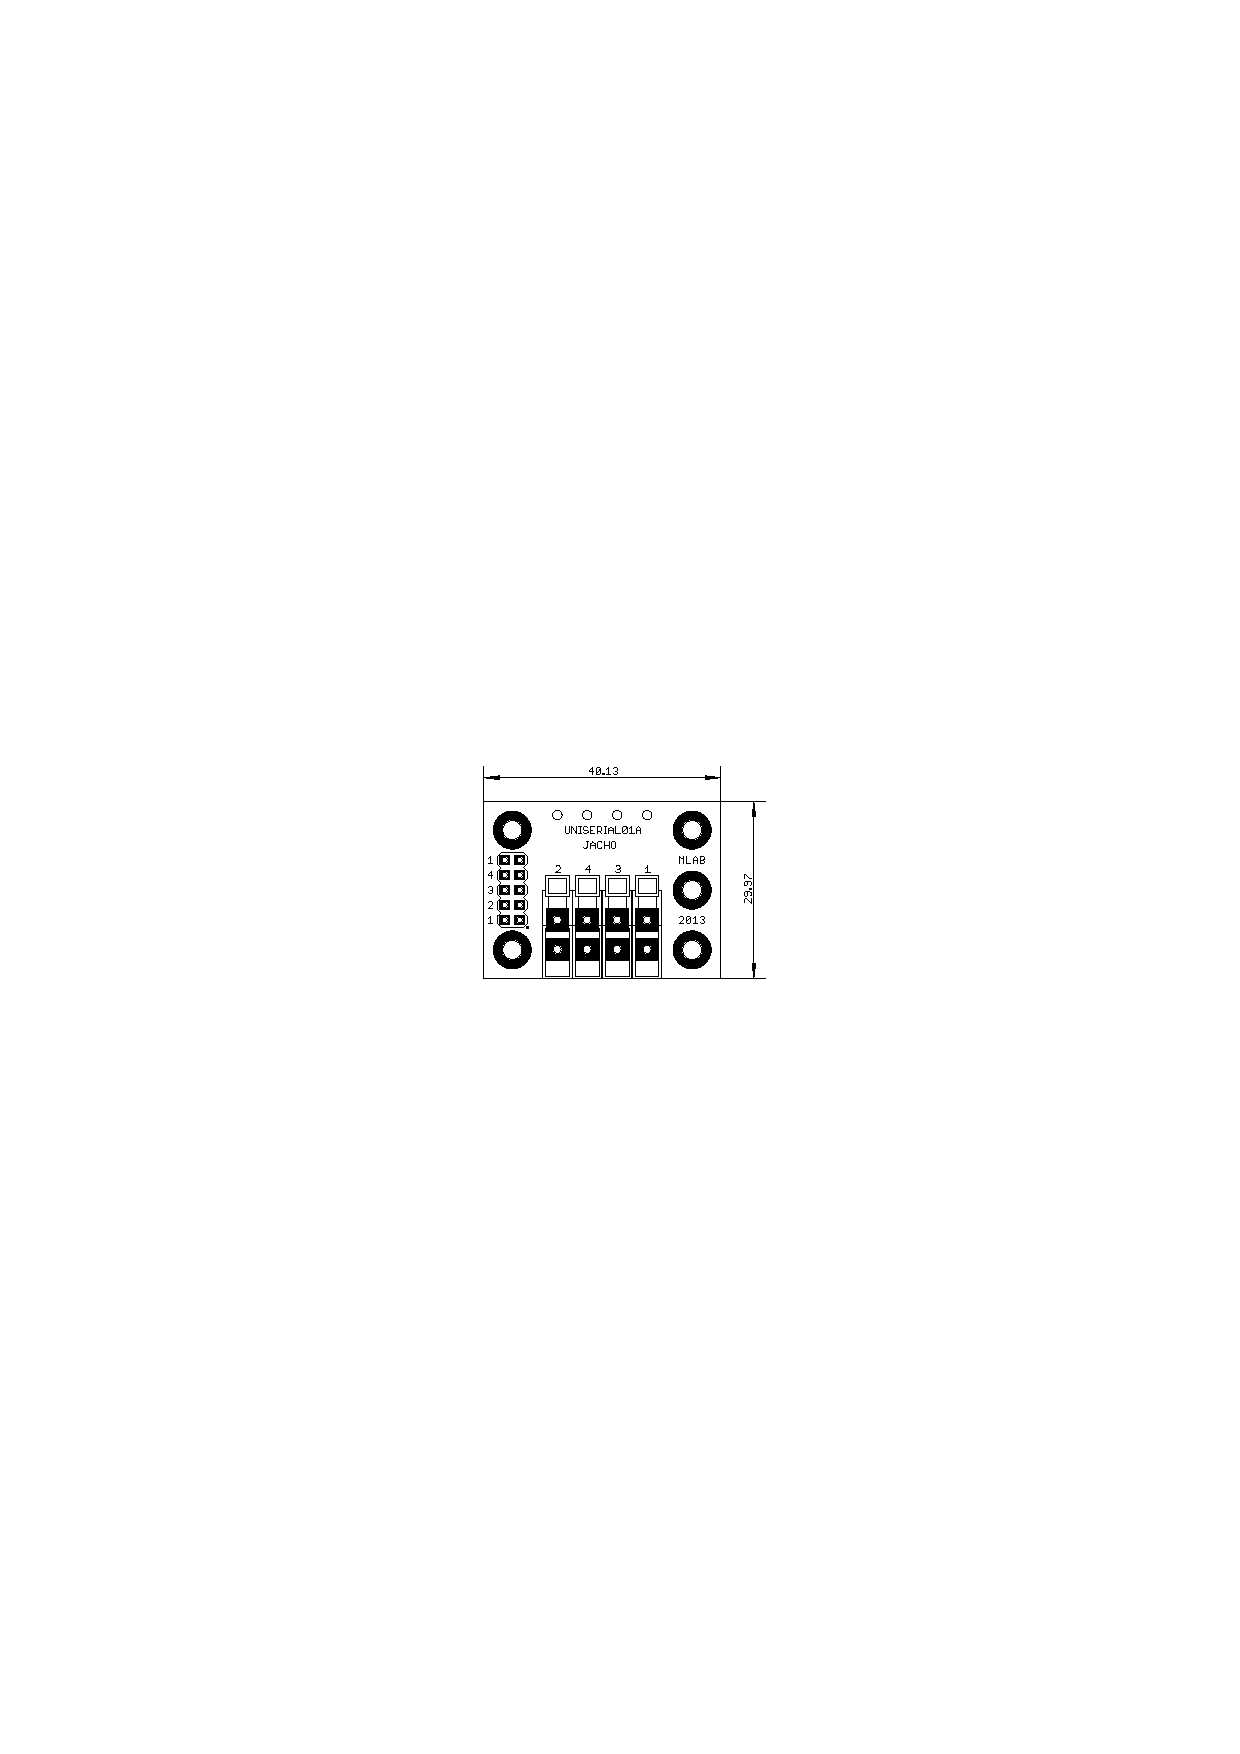
\includegraphics[trim = 8.0cm 11.5cm 8.0cm 11.5cm, clip, width=10cm]{../../CAM_DOC/O1.pdf}
  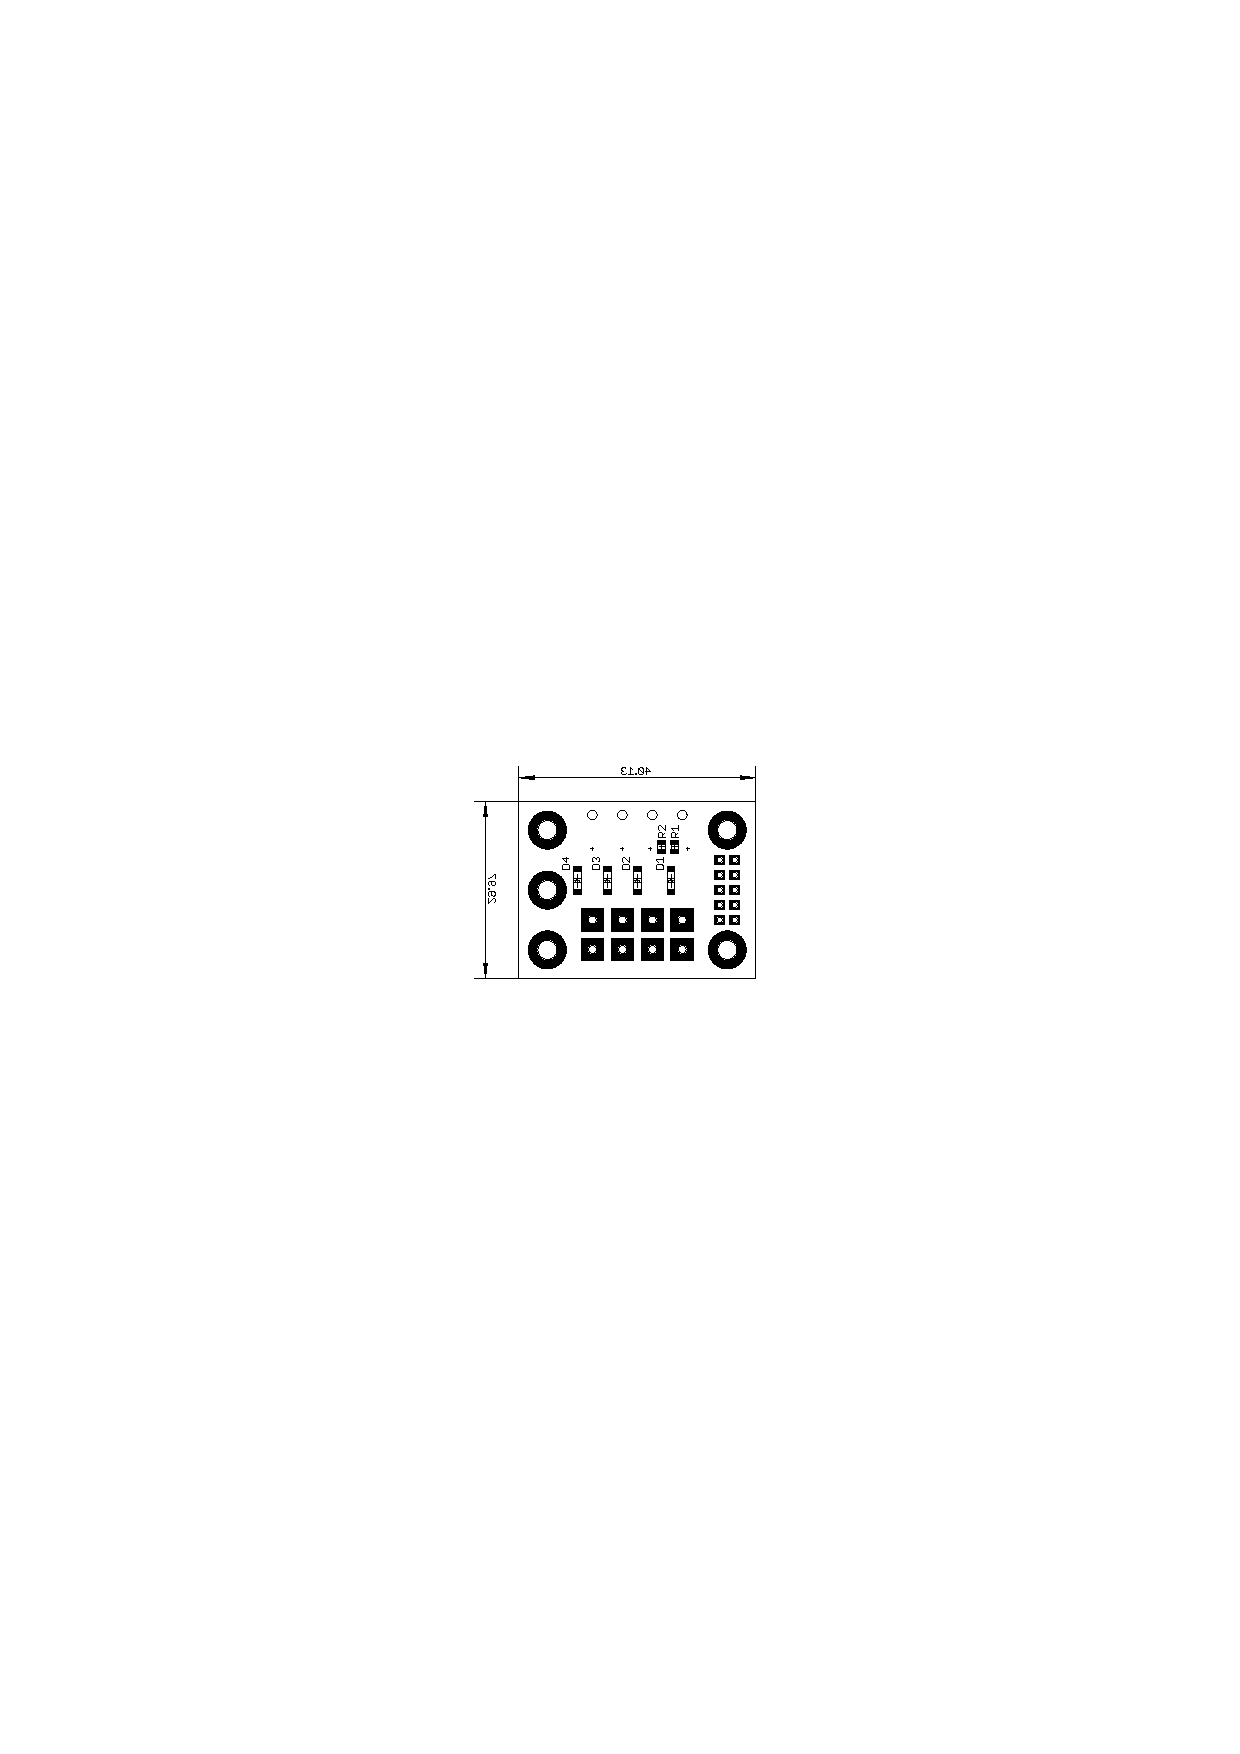
\includegraphics[trim = 8.0cm 11.5cm 8.0cm 11.5cm, clip, width=10cm]{../../CAM_DOC/O2.pdf}
  \caption{Osazovací plán horní a spodní strany plošného spoje}
  \label{fig:osazovaci_plan}
\end{figure}

\begin{thebibliography}{99}
%\bibitem{DR2G}{Původní konstrukce} 
%\href{http:// odkaz na nejakou zajimavou konstrukci}{odkaz na nejakou zajimavou konstrukci}

\end{thebibliography}
\end{document}